%%%%%%%%%%%%%%%%%%%%%%%%%%%%%%%%%%%%%%%%%%%%%%%%%%%%%
% SPARSE SYNTHETIC CONTROL
%%%%%%%%%%%%%%%%%%%%%%%%%%%%%%%%%%%%%%%%%%%%%%%%%%%%%
\subsection{Sparse Synthetic Control}

The core component of our pairs trading strategy involves constructing a synthetic asset that replicates the price behavior of a target security using a sparse combination of assets from a donor pool. 
%
Let $\mathcal T$ denote the collection of timestamps of a time series with $T:=\card{\mathcal T}$. This sample is divided into training and test samples: $\mathcal T=\mathcal T_{tr} \cup \mathcal T_{test}$.\footnote{Throughout the text, we will indisctinctively refer to the training sample as \qquote{estimation sample} or as \qquote{in-sample}. Analogously, we will refer to the test sample as the \qquote{evaluation sample} or more succintly, \qquote{out-of-sample}}
%
Let $\mbf y = [y_{t}]_{t=1}^T\in \R^{T}$ denote the log-price time series of a target asset and $\mbf X = [x_{1t}, ..., x_{Nt}]_{t=1}^T\in\R^{T\times N}$ denote the log-price time series of a donor pool of assets. Then, we can build a synthetic asset time series ${\mbf y}^*$ as
\begin{equation*}
{y}_{t}^* = \sum_{i=1}^N w_i^* x_{it}
\quad \text{for~} t=1,...,T
,
\end{equation*}

where the weights $\mbf w^*=[w_1^*, ..., w_N^*]\'\in \R^N$ are determined in-sample via an $\ell_1$-regularized least squares optimization problem
%----------------------------------------------------
\begin{equation*}
\mathbf{w}^* 
= \argmin_{\mathbf{w} \in \R^{N}} \left\{\sum_{t\in\mathcal T_{tr}} \left(y_{t} - \sum_{i=1}^N w_i x_{it}\right)^2 + \lambda\|\mathbf{w}\|_1\right\}
\quad \text{s.t.} \quad \mathbf{1}^\top \mathbf{w} = 1
\end{equation*}
%----------------------------------------------------
%\begin{equation*}
%\mathbf{w}^* 
%= 
%\2{
%\begin{array}{cl}
%\underset{\mathbf{w} \in \R^{N}}{\arg\min} &
%\sum_{t=1}^T \left(y_{t} - \sum_{i=1}^N w_i x_{it}\right)^2 
%%\norm{\mbf y - \mbf {Xw}}_2^2
%+ \lambda\|\mathbf{w}\|_1
%\\
%\text{s.t.} & \mathbf{1}^\top \mathbf{w} = 1
%\end{array}
%}
%\end{equation*}
%----------------------------------------------------

where $\|\mathbf{w}\|_1 = \sum_{i=1}^N |w_i|$ denotes the $\ell_1$-norm of the weight vector, $\lambda > 0$ is a regularization parameter that controls the level of sparsity.
%This formulation promotes sparse solutions through the $\ell_1$ penalty term while maintaining the constraint that the weights sum to unity. 
The $\ell_1$ regularization, also known as the lasso penalty, induces sparsity by shrinking some weights exactly to zero, effectively performing feature selection among the donor assets. This sparsity-inducing property stems from the non-differentiability of the penalty term at the origin. %\cite{tibshirani1996regression}.
The practical implementation of this procedure is given in \cref{alg:synthetic_control}

The optimization problem possesses several key theoretical and practical features that make it particularly suitable for our application. First, the combination of a quadratic loss function with the convex $\ell_1$-penalty and affine constraint guarantees a unique solution under mild regularity conditions. % \cite{boyd2004convex}.
Second, the regularization parameter $\lambda$ (optimally selected through cross-validation) provides direct control over the sparsity level, with larger values yielding solutions with fewer non-zero weights. Third, the simplex constraint $\mbf 1^\top \mbf w = 1$ ensures interpretability of the synthetic control as a weighted portfolio of donor assets. We don't impose a convex hull restriction, which effectively means that we allow for negative ways in the synthetic asset.

The resulting weight vector $\mathbf{w}^*$ will typically have many components equal or very close to zero, with the number of non-zero weights decreasing as $\lambda$ increases. In practice, we identify the support of non-zero weights through thresholding:
\begin{equation*}
\mathcal{I} = \{i \in \{1,...,N\} : |w^*_i| > \epsilon\}
\end{equation*}
where $\epsilon > 0$ is a small tolerance threshold (in our application, $\epsilon \approx 10^{-5}$). The final synthetic asset is then constructed using only assets in $\mathcal{I}$. We chose to sparsify the synthetic control using lasso instead of solving a cardinality-constrained program as the former is able to maintain sparse exposures while enjoying vast computational advantages. Moreover, the convex nature of the problem permits efficient solution via proximal algorithms or quadratic programming techniques, making it suitable for high-dimensional donor pools. For a detailed discussion, see \cref{sec:discussion_card_constr}.


The reader may draw similarities of this process with the Engle-Granger procedure for estimating the cointegration vector associated to the target asset and the donor pool. If we don't impose the $\ell_1$-penalty, it can be shown that, under some conditions, the procedure of finding the weights of the synthetic control is equivalent to finding the cointegration vector. For a formal discussion see \cref{sec:cointegration_meets_synthetic_controls}.


%==============[	  Empirical Application  ]==============
%For the empirical application, we will use daily adjusted-close stock price data from the S\&P500. For illustration, we will set NVIDIA as our target stock and leave all the rest stocks in the donor pool. We have data from January 2010 to January 2025. We divide it into training ($70\%$) and test set ($30\%$) and obtain the synthetic control weights from the training sample. This delivers the weights shown in \cref{tab:scm_weights}. As we can see, our synthetic control is composed of 27 stocks with weights that sum to 1. Some weights are positive, indicating a long position, and others are negative, indicating a short position. 
%This sparse portfolio structure effectively defines a tradeable basket that can be executed simultaneously through standard ETF-like basket trading mechanisms.
%This synthetic control defines a \qquote{basket} that is to be traded at unison in an ETF-like style.

To evaluate our methodology empirically, we implement the synthetic control approach using daily adjusted-close price data from S\&P500 constituents. We select NVIDIA (NVDA) as our target asset and construct the donor pool from the remaining index components. The full sample runs from January 2010 to January 2025 and is partitioned chronologically, with 70\% allocated to the training period for model estimation and the remaining 30\% reserved for out-of-sample testing. The optimization procedure detailed in the previous section yields the optimal weights presented in \cref{tab:scm_weights}. The resulting synthetic control comprises 27 stocks with non-zero weights that sum to unity, distributed between long positions (positive weights) and short positions (negative weights). This sparse portfolio structure effectively defines a tradeable basket that can be executed simultaneously through standard ETF-like basket trading mechanisms.

%==============[	  Table 1 ]==============
\begin{table}[H] 
\centering
\caption{Synthetic Control Model Weights}
\label{tab:scm_weights}
\begin{tabular}{llc}
\toprule
 Tickers & Company Name & Weights (\%) \\
\midrule
\textbf{AME} & Ametek & 41.08 \\
\textbf{LUV} & Southwest Airlines & 33.31 \\
\textbf{TFC} & Truist Financial & 25.60 \\
\textbf{AEP} & American Electric Power & 21.69 \\
\textbf{ADM} & Archer Daniels Midland & 20.56 \\
\textbf{RSG} & Republic Services & 18.42 \\
\textbf{AXP} & American Express & 18.10 \\
\textbf{LLY} & Lilly (Eli) & 14.74 \\
\textbf{C} & Citigroup & 9.67 \\
\textbf{VRSN} & Verisign & 7.77 \\
\textbf{MTB} & M\&T Bank & 7.38 \\
\textbf{FE} & FirstEnergy & 7.16 \\
\textbf{FIS} & Fidelity National Information Services & 5.21 \\
\textbf{PARA} & Paramount Global & 4.48 \\
\textbf{TXT} & Textron & 2.21 \\
\textbf{STX} & Seagate Technology & 0.26 \\
\textbf{BIIB} & Biogen & 0.16 \\
\textbf{NFLX} & Netflix & -1.04 \\
\textbf{FDX} & FedEx & -2.39 \\
\textbf{UDR} & UDR, Inc. & -3.95 \\
\textbf{V} & Visa Inc. & -5.43 \\
\textbf{CNP} & CenterPoint Energy & -7.75 \\
\textbf{MS} & Morgan Stanley & -16.21 \\
\textbf{NI} & NiSource & -16.35 \\
\textbf{WMT} & Walmart & -16.65 \\
\textbf{UNP} & Union Pacific Corporation & -25.77 \\
\textbf{ADSK} & Autodesk & -42.25 \\
\bottomrule
 & Total& 100.00 \\
\bottomrule
\end{tabular}

%----------------------------------------------------
\vspace{0.5cm}
\begin{minipage}{\textwidth}
\setlength{\parindent}{0pt}
\small\textit{Note: 
% Optimal weights of the sparse synthetic control portfolio for replicating the target asset's price dynamics. The table displays the percentage contribution of each donor asset from the S\&P 500 constituents, with positive weights indicating long positions and negative weights indicating short positions. The weights are derived using an $\ell_1$-regularized least squares optimization, which enforces sparsity by shrinking some weights to zero, effectively selecting the most influential assets. The weights sum to 100\% as enforced by the simplex constraint in the optimization problem.
This table presents the optimal weights obtained from the sparse synthetic control methodology for replicating the target asset's price dynamics. The weights are expressed as percentages and represent each donor asset's contribution to the synthetic portfolio. Positive weights indicate long positions while negative weights represent short positions. The donor pool consists of S\&P 500 constituents, and the methodology yields a sparse solution where many potential donor assets receive zero weights. The sparsity is achieved through $\ell_1$-regularization, which automatically selects the most influential assets for constructing the synthetic control. The weights sum to 100\% as enforced by the simplex constraint in the optimization problem.
}
\end{minipage}
%----------------------------------------------------
\end{table}


%%%%%%%%%%%%%%%%%%%%%%%%%%%%%%%%%%%%%%%%%%%%%%%%%%%%%
%%%%%%%%%%%%%%%%%%%%%%%%%%%%%%%%%%%%%%%%%%%%%%%%%%%%%
%\inserthere{tab:scm_weights}
%\begin{table}[H] 
%\centering
%\caption{Synthetic Control Model Weights}
%\label{tab:scm_weights}
%\begin{tabular}{cc}
%\toprule
% Tickers & Weights (\%) \\
%\midrule
%\textbf{AME} & 41.08 \\
%\textbf{LUV} & 33.31 \\
%\textbf{TFC} & 25.60 \\
%\textbf{AEP} & 21.69 \\
%\textbf{ADM} & 20.56 \\
%\textbf{RSG} & 18.42 \\
%\textbf{AXP} & 18.10 \\
%\textbf{LLY} & 14.74 \\
%\textbf{C} & 9.67 \\
%\textbf{VRSN} & 7.77 \\
%\textbf{MTB} & 7.38 \\
%\textbf{FE} & 7.16 \\
%\textbf{FIS} & 5.21 \\
%\textbf{PARA} & 4.48 \\
%\textbf{TXT} & 2.21 \\
%\textbf{STX} & 0.26 \\
%\textbf{BIIB} & 0.16 \\
%\textbf{NFLX} & -1.04 \\
%\textbf{FDX} & -2.39 \\
%\textbf{UDR} & -3.95 \\
%\textbf{V} & -5.43 \\
%\textbf{CNP} & -7.75 \\
%\textbf{MS} & -16.21 \\
%\textbf{NI} & -16.35 \\
%\textbf{WMT} & -16.65 \\
%\textbf{UNP} & -25.77 \\
%\textbf{ADSK} & -42.25 \\
%\bottomrule
%\textbf{Total} & 100.00 \\
%\bottomrule
%\end{tabular}
%
%%----------------------------------------------------
%\vspace{0.5cm}
%\begin{minipage}{\textwidth}
%\setlength{\parindent}{0pt}
%\small\textit{Note: 
%% Optimal weights of the sparse synthetic control portfolio for replicating the target asset's price dynamics. The table displays the percentage contribution of each donor asset from the S\&P 500 constituents, with positive weights indicating long positions and negative weights indicating short positions. The weights are derived using an $\ell_1$-regularized least squares optimization, which enforces sparsity by shrinking some weights to zero, effectively selecting the most influential assets. The weights sum to 100\% as enforced by the simplex constraint in the optimization problem.
%This table presents the optimal weights obtained from the sparse synthetic control methodology for replicating the target asset's price dynamics. The weights are expressed as percentages and represent each donor asset's contribution to the synthetic portfolio. Positive weights indicate long positions while negative weights represent short positions. The donor pool consists of S\&P 500 constituents, and the methodology yields a sparse solution where many potential donor assets receive zero weights. The sparsity is achieved through $\ell_1$-regularization, which automatically selects the most influential assets for constructing the synthetic control. The weights sum to 100\% as enforced by the simplex constraint in the optimization problem.
%}
%\end{minipage}
%%----------------------------------------------------
%\end{table}



The time series evolution of the target and synthetic log-prices is shown in \cref{fig:target_synthetic_prices_NVDA}. As we can see, the fit is really good in the training sample, but as we move out of sample, the spread between the two series becomes more volatile and the two series seem to diverge in recent years. As we will see later, we should not worry too much about the log-price fit, as the trading strategy capitalizes on the mean-reversion of returns (rather than log-prices).

%==============[	  Figure 1  ]==============
\inserthere{fig:target_synthetic_prices_NVDA}
\begin{figure}[H]
  \caption{Target vs Synthetic Log-Prices for NVDA}
  \centering
  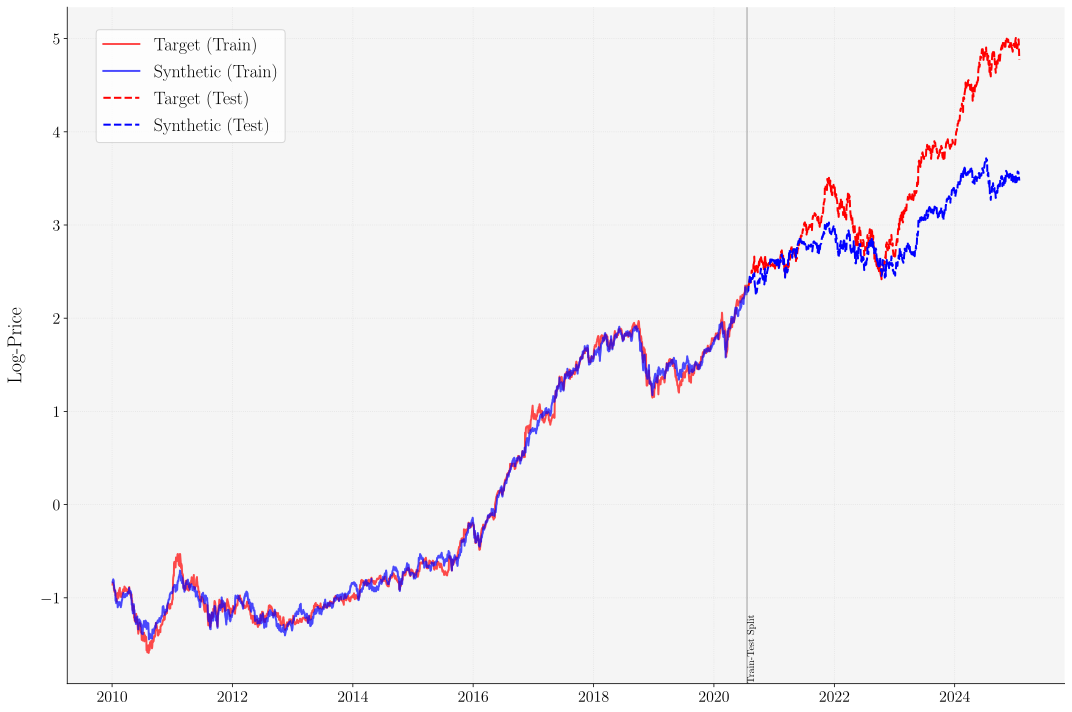
\includegraphics[scale=0.47]{/Users/jesusvillotamiranda/Library/CloudStorage/OneDrive-UniversidaddeLaRioja/GitHub/Repository/arbitragelab-master/__OUTPUT_TeX__/figures/target_synthetic_prices_NVDA.pdf}
\label{fig:target_synthetic_prices_NVDA}
%.............
\vspace{0.5cm}
\begin{minipage}{\textwidth}
\setlength{\parindent}{0pt}
\small\textit{Note: 
This figure illustrates the log-price trajectories of the target asset (NVDA) and its synthetic counterpart over the training and testing periods. The solid blue line represents the synthetic log-prices derived from the sparse synthetic control methodology, while the solid red line indicates the actual log-prices of the target asset during the training phase. The dashed lines depict the log-prices for both the target and synthetic assets during the testing phase. The vertical line marks the transition point between the training and testing datasets
}
\end{minipage}
%.............
\end{figure}



%%%%%%%%%%%%%%%%%%%%%%%%%%%%%%%%%%%%%%%%%%%%%%%%%%%%%%
%% SPARSE SYNTHETIC CONTROL
%%%%%%%%%%%%%%%%%%%%%%%%%%%%%%%%%%%%%%%%%%%%%%%%%%%%%%
%\subsection{Sparse Synthetic Control}
%
%The core component of our pairs trading strategy involves constructing a synthetic asset that replicates the price behavior of a target security (e.g: AAPL) using a sparse combination of assets from a donor pool. 
%Let $\mbf y = [y_{t}]_{t=1}^T\in \R^{T}$ denote the log-price time series of a target asset and $\mbf X = [x_{1t}, ..., x_{Nt}]_{t=1}^T\in\R^{T\times N}$ denote the log-price time series of a donor pool of assets. Then, we can build a synthetic asset ${\mbf y}^*$ as\begin{equation*}
%{y}_{t}^* = \sum_{i=1}^N w_i^* x_{it}
%,
%\end{equation*}
%
%where the weights $\mbf w^*=[w_1^*, ..., w_N^*]\'$ are determined via an $\ell_1$-regularized least squares optimization problem
%
%\begin{equation*}
%\mathbf{w}^* = \argmin_{\mathbf{w} \in \R^{N}} \left\{\sum_{t=1}^T \left(y_{t} - \sum_{i=1}^N w_i x_{it}\right)^2 + \lambda\|\mathbf{w}\|_1\right\}
%\quad \text{s.t.} \quad \mathbf{1}^\top \mathbf{w} = 1
%\end{equation*}
%where $\|\mathbf{w}\|_1 = \sum_{i=1}^N |w_i|$ denotes the $\ell_1$-norm of the weight vector and $\lambda > 0$ is a regularization parameter that controls the level of sparsity. This formulation promotes sparse solutions through the $\ell_1$ penalty term while maintaining the constraint that the weights sum to unity. The $\ell_1$ regularization, also known as the lasso penalty, induces sparsity by shrinking some weights exactly to zero, effectively performing feature selection among the donor assets.
%\bblue{The $\ell_1$-penalty induces sparsity by shrinking small weights to zero through the non-differentiability of the penalty term at the origin \cite{tibshirani1996regression}}
%
%The optimization problem is convex and can be efficiently solved using standard convex optimization algorithms. The resulting weight vector $\mathbf{w}^*$ will typically have many components exactly equal to zero, with the number of non-zero weights decreasing as $\lambda$ increases. This provides a computationally tractable approach to constructing sparse synthetic controls, where only a subset of the donor assets contribute to replicating the target asset's behavior.
%
%
%For a discussion of the formal equivalence of this procedure with cointegration analysis, see \cref{sec:cointegration_meets_synthetic_controls}.
%
%
%\bblue{
%The optimization problem possesses several key features:
%
%\begin{itemize}
%\item \textbf{Convexity}: The quadratic loss function combined with the convex $\ell_1$-penalty and affine constraint guarantees a unique solution under mild regularity conditions \cite{boyd2004convex}.
%
%\item \textbf{Sparsity Control}: The regularization parameter $\lambda$ governs the number of non-zero weights, with larger values yielding sparser solutions. Optimal $\lambda$ selection can be performed via cross-validation or information criteria.
%
%\item \textbf{Portfolio Interpretation}: The simplex constraint $\mbf 1^\top \mbf w = 1$ ensures interpretability as a weighted portfolio of donor assets. Note that we are not imposing a convex hull restriction (which would restrict donor weights to be nonnegative). 
%\end{itemize}
%
%Post-optimization, the support of non-zero weights is identified through thresholding:
%\begin{equation*}
%\mathcal{I} = \{i \in \{1,...,N\} : |w^*_i| > \epsilon\}
%\end{equation*}
%
%where $\epsilon > 0$ is a small tolerance threshold (in our application, $\epsilon \approx 10^{-6}$). The final synthetic asset is then constructed using only assets in $\mathcal{I}$. %, effectively automating donor selection through continuous optimization rather than combinatorial search.
%%
%This approach provides computational advantages over cardinality-constrained formulations while maintaining sparse exposures. The convex formulation permits efficient solution via proximal algorithms or quadratic programming techniques, making it suitable for high-dimensional donor pools \cite{beck2009fast}.
%}

%%%%%%%%%%%%%%%%%%%%%%%%%%%%%%%%%%%%%%%%%%%%%%%%%%%%%%%
%% SPARSE SYNTHETIC CONTROL
%%%%%%%%%%%%%%%%%%%%%%%%%%%%%%%%%%%%%%%%%%%%%%%%%%%%%%
%\subsection{Sparse Synthetic Control}
%
%The core component of our pairs trading strategy involves constructing a synthetic asset that replicates the price behavior of a target security (e.g., AAPL) using a combination of assets from a donor pool.
%Let $\mbf y = [y_{t}]_{t=1}^T\in \R^{T}$ denote the log-price time series of a target asset and $\mbf X = [x_{1t}, ..., x_{Nt}]_{t=1}^T\in\R^{T\times N}$ denote the log-price time series of a donor pool of assets. We construct a synthetic asset ${\mbf y}^*$ through a sparse linear combination
%\begin{equation*}
%{y}_{t}^* = \sum_{i=1}^N w_i^* x_{it}
%.
%\end{equation*}
%%
%The weights $\mbf w^*=[w_1^*, ..., w_N^*]$ are determined via an L1-regularized quadratic program
%%
%\begin{equation*}
%\mathbf{w}^* = \argmin_{\mathbf{w} \in \R^{N}} \sum_{t=1}^T \left(y_{t} - \sum_{i=1}^N w_i x_{it}\right)^2 + \lambda \sum_{i=1}^N |w_i|
%\quad \text{s.t.} \quad
%\mbf 1\' \mbf w = 1
%.
%\end{equation*}
%%
%where $\lambda$ is a regularization parameter that controls the sparsity of the solution. The L1 penalty term $\sum_{i=1}^N |w_i|$ promotes sparsity by encouraging many of the weights to be exactly zero, thereby selecting only a limited number of assets to receive nonzero weights.
%%
%%
%%
%%
%The L1-regularized optimization problem is solved using the following procedure:
%\begin{enumerate}
%\item Define the decision variable $\mbf w \in \R^N$.
%\item Formulate the objective function as the sum of the least squares error and the L1 penalty:
%%
%\begin{equation*}
%\text{Objective} = \sum_{t=1}^T \left(y_{t} - \sum_{i=1}^N w_i x_{it}\right)^2 + \lambda \sum_{i=1}^N |w_i|.
%\end{equation*}
%%
%\item Impose the constraint that the weights sum to 1:
%%
%\begin{equation*}
%\mbf 1\' \mbf w = 1.
%\end{equation*}
%%
%\item Solve the optimization problem using a convex optimization solver to obtain the optimal weights $\mbf w^*$.
%\end{enumerate}
%%
%The resulting weights $\mbf w^*$ are then used to construct the synthetic asset ${\mbf y}^*$ as follows:
%\begin{equation*}
%{y}_{t}^* = \sum_{i=1}^N w_i^* x_{it}.
%\end{equation*}
%%
%This approach ensures that the synthetic asset closely replicates the target asset while maintaining sparsity in the selection of donor assets.



%%%%%%%%%%%%%%%%%%%%%%%%%%%%%%%%%%%%%%%%%%%%%%%%%%%%%
% SPARSE SYNTHETIC CONTROL VIA L1 REGULARIZATION
%%%%%%%%%%%%%%%%%%%%%%%%%%%%%%%%%%%%%%%%%%%%%%%%%%%%%
\subsection{Sparse Synthetic Control via $\ell_1$-Regularization}

The synthetic asset construction employs an $\ell_1$-regularized convex optimization approach to simultaneously achieve portfolio sparsity and tracking accuracy. Let $\mbf y = [y_{t}]_{t=1}^T\in \R^{T}$ denote the log-price trajectory of the target asset and $\mbf X = [x_{1t}, ..., x_{Nt}]_{t=1}^T\in\R^{T\times N}$ represent the log-prices of $N$ assets in the donor pool. We construct a synthetic asset ${y}^*_t$ through a sparse linear combination:

\begin{equation*}
{y}^*_t = \sum_{i=1}^N w^*_i x_{it}
\end{equation*}

The weight vector $\mbf w^* = [w^*_1, ..., w^*_N]^\top$ is determined by solving the following convex optimization problem:

\begin{equation}
\mbf w^* = \argmin_{\mbf w \in \R^N} \left\{ \underbrace{\sum_{t=1}^T \left(y_t - \sum_{i=1}^N w_i x_{it}\right)^2}_{\text{Tracking error}} + \lambda \underbrace{\sum_{i=1}^N |w_i|}_{\ell_1\text{-penalty}} \right\} \quad \text{s.t.} \quad \mbf 1^\top \mbf w = 1
\end{equation}

where $\lambda > 0$ is a regularization parameter controlling the sparsity-accuracy trade-off. The $\ell_1$-penalty induces sparsity by shrinking small weights to zero through the non-differentiability of the penalty term at the origin \cite{tibshirani1996regression}. This convex relaxation avoids the computational complexity of cardinality constraints while maintaining desirable sparsity properties.

The optimization problem possesses several key features:

\begin{itemize}
\item \textbf{Convexity}: The quadratic loss function combined with the convex $\ell_1$-penalty and affine constraint guarantees a unique solution under mild regularity conditions \cite{boyd2004convex}.

\item \textbf{Sparsity Control}: The regularization parameter $\lambda$ governs the number of non-zero weights, with larger values yielding sparser solutions. Optimal $\lambda$ selection can be performed via cross-validation or information criteria.

\item \textbf{Portfolio Interpretation}: The simplex constraint $\mbf 1^\top \mbf w = 1$ ensures interpretability as a weighted portfolio of donor assets, preventing leverage through short positions.
\end{itemize}

Post-optimization, the support of non-zero weights is identified through thresholding:

\begin{equation*}
\mathcal{I} = \{i \in \{1,...,N\} : |w^*_i| > \epsilon\}
\end{equation*}

where $\epsilon > 0$ is a small tolerance threshold (typically $\epsilon \approx 10^{-6}$). The final synthetic asset is then constructed using only assets in $\mathcal{I}$, effectively automating donor selection through continuous optimization rather than combinatorial search.

This approach provides computational advantages over cardinality-constrained formulations while maintaining sparse exposures. The convex formulation permits efficient solution via proximal algorithms or quadratic programming techniques, making it suitable for high-dimensional donor pools \cite{beck2009fast}.


%%%%%%%%%%%%%%%%%%%%%%%%%%%%%%%%%%%%%%%%%%%%%%%%%%%%%
% SPARSE SYNTHETIC CONTROL
%%%%%%%%%%%%%%%%%%%%%%%%%%%%%%%%%%%%%%%%%%%%%%%%%%%%%
\subsection{Sparse Synthetic Control}

The core component of our pairs trading strategy involves constructing a synthetic asset that replicates the price behavior of a target security (e.g., AAPL) using a combination of assets from a donor pool. Let $\mbf y = [y_{t}]_{t=1}^T\in \R^{T}$ denote the log-price time series of a target asset and $\mbf X = [x_{1t}, ..., x_{Nt}]_{t=1}^T\in\R^{T\times N}$ denote the log-price time series of a donor pool of assets. We construct a synthetic asset ${\mbf y}^*$ through a sparse linear combination
\begin{equation*}
{y}_{t}^* = \sum_{i=1}^N w_i^* x_{it},
\end{equation*}
where the weights $\mbf w^*=[w_1^*, ..., w_N^*]$ are determined by solving an L1-regularized optimization problem. This approach promotes sparsity in the weights, ensuring that only a limited number of assets from the donor pool contribute to the synthetic asset.

Specifically, we solve the following convex optimization problem:
\begin{equation*}
\mathbf{w}^* = \argmin_{\mathbf{w} \in \R^{N}} \norm{\mathbf{y} - \mathbf{X}\mathbf{w}}_2^2 + \lambda \norm{\mathbf{w}}_1 
\quad \text{s.t.} \quad 
\mbf 1^\top \mbf w = 1,
\end{equation*}
where $\lambda > 0$ is a regularization parameter that controls the trade-off between sparsity and reconstruction accuracy. The term $\norm{\mathbf{w}}_1 := \sum_{i=1}^N |w_i|$ represents the L1-norm, which induces sparsity in the solution by penalizing nonzero weights.

This formulation has several advantages:
- The optimization problem is convex, ensuring computational efficiency and global optimality.
- The L1 penalty enforces sparsity directly, eliminating the need for heuristic approximations to cardinality constraints.
- The resulting weights are interpretable and robust, as only a subset of donor assets with significant contributions are selected.

The solution is obtained using numerical solvers for convex optimization, and assets with weights below a small threshold (e.g., $10^{-6}$) are effectively treated as having zero contribution. This approach provides a principled and rigorous framework for constructing sparse synthetic controls in pairs trading applications.



%%%%%%%%%%%%%%%%%%%%%%%%%%%%%%%%%%%%%%%%%%%%%%%%%%%%%
% SPARSE SYNTHETIC CONTROL VIA L1 REGULARIZATION
%%%%%%%%%%%%%%%%%%%%%%%%%%%%%%%%%%%%%%%%%%%%%%%%%%%%%
\subsection{Sparse Synthetic Control via \texorpdfstring{$L^1$}{L1} Regularization}

The synthetic asset construction problem is formulated as a convex optimization program with sparsity-inducing regularization. Let $\mbf y = [y_{t}]_{t=1}^T\in \R^{T}$ denote the log-price trajectory of the target asset and $\mbf X = [x_{1t}, ..., x_{Nt}]_{t=1}^T\in\R^{T\times N}$ the log-price matrix of the donor assets. We construct the synthetic asset $\mbf y^*$ through:

\begin{equation*}
{y}_{t}^* = \sum_{i=1}^N w_i^* x_{it}
\end{equation*}

The weights $\mbf w^*\in \R^N$ are determined via the regularized quadratic program:

\begin{equation*}
\mathbf{w}^* = \argmin_{\mathbf{w} \in \R^{N}} \left[ \underbrace{\sum_{t=1}^T \left(y_{t} - \sum_{i=1}^N w_i x_{it}\right)^2}_{\text{Tracking Error}} + \lambda \underbrace{\sum_{i=1}^N |w_i|}_{\text{$L^1$ Regularizer}} \right]
\quad \text{s.t.} \quad 
\left|
\begin{array}{ll}
	\mbf 1^\top \mbf w &= 1 
\end{array}
\right.
\end{equation*}

Where:
\begin{itemize}
\item $\lambda > 0$ is a hyperparameter controlling sparsity-intensity tradeoff
\item The $L^1$ regularizer induces parsimony through the geometric properties of the 1-norm ball
\item The simplex constraint $\mbf 1^\top \mbf w = 1$ ensures interpretable portfolio weights
\end{itemize}

This convex relaxation of the NP-hard cardinality-constrained problem provides:
\begin{itemize}
\item \textbf{Global optimality}: Elimination of local minima through convexity
\item \textbf{Sparsity}: The $L^1$ term shrinks small weights to zero via exact penalization
\item \textbf{Computational efficiency}: Enables use of convex optimization algorithms
\end{itemize}

The optimal weights $\mbf w^*$ satisfy the first-order Karush-Kuhn-Tucker conditions:
\begin{equation*}
\mbf X^\top(\mbf y - \mbf X\mbf w^*) = \frac{\lambda}{2}\mbf s + \mu\mbf 1
\end{equation*}
where $\mbf s \in \{-1,0,1\}^N$ is the subgradient of $\|\mbf w^*\|_1$ and $\mu$ is the Lagrange multiplier for the budget constraint.

The sparse support set $\mathcal{I} := \{i \in [N] : w_i^* \neq 0\}$ emerges endogenously from the optimization, with cardinality controlled by $\lambda$. Larger $\lambda$ values yield sparser solutions through more aggressive weight shrinkage, as shown by the regularization path:

\begin{equation*}
|\mbf X_i^\top(\mbf y - \mbf X\mbf w^*)| \leq \frac{\lambda}{2} + \mu \quad \forall i \notin \mathcal{I}
\end{equation*}

This formulation maintains the synthetic asset's economic interpretation as a statistical arbitrage portfolio while achieving parsimony through modern regularization techniques.


%==============[	  DISCUSSION  ]==============

%Many alternative procedures for building a sparse synthetic control can be devised. A natural one would be to directly perform a cardinality constrained quadratic program 
%\begin{equation*}
%\mathbf{w}^* = \argmin_{\mathbf{w} \in \R^{N}} \sum_{t=1}^T \left(y_{t} - \sum_{i=1}^N w_i x_{it}\right)^2 
%\quad \text{s.t.} \quad 
%\left|
%\begin{array}{ll}
%	\mbf 1\' \mbf w &= 1 \\
%	\norm{\mathbf{w}}_0 &\leq K
%\end{array}
%\right
%.
%\end{equation*}
%%
%where $\|\mathbf{w}\|_0:=\sum_{i=1}^N \I{w_i\neq 0}$ counts the non-zero elements in $\mbf w$. The goal is to enforce sparsity so that only a limited number of assets receive a nonzero weight. 
%%
%%
%%
%%
%The NP-hard cardinality constraint can be approximated by many different procedures:
%
%\subsubsection{Mixed integer} % mixed integer stuff here
%% explain this in detail
%
%\subsubsection{Procedure 2} % Give a name to this procedure 
%\begin{enumerate}
%\item Solve the full least squares problem
%%
%\begin{equation*}
%\mathbf{w}^{(1)} = \argmin_{\mathbf{w} \in \mathbb{R}^{N}} \norm{\mathbf{y} - \mathbf{X}\mathbf{w}}_2^2
%\quad \text{s.t.} \quad \mathbf{1}^\top \mbf w=1.
%\end{equation*}
%%
%\item Select the $K$ largest weights (in absolute value) from $\mbf w^{(1)}$ into
%$$\mathcal I:=\{i : |w_i^{(1)}| \t{~among $K$ largests}\}$$
%%
%\item Solve the restricted program on support $\mathcal I$
%%
%\begin{equation*}
%	\mbf w^{(2)} = \arg \min_{\mbf w_{\mathcal I}\in \mathbb{R}^K} \norm{\mbf y - \mbf X_{\mathcal I}\mbf w_{\mathcal I}}_{2}^{2}
%\quad \text{s.t.} \quad 
%\mbf 1\' \mbf w_{\mathcal I} = 1
%\end{equation*}
%%
%where $\mbf X_{\mathcal{I}} \in \mathbb{R}^{T \times K}$ is the resricted donor matrix and $\mbf w_{\mathcal{I}} \in \mathbb{R}^{K}$ is the restricted weight vector for the selected assets.
%%
%\item Construct the full weight vector $\mbf w^* \in \mathbb{R}^{N}$ by embedding the optimized restricted weights back into the original $N$-dimensional space. 
%\begin{equation*}
%	w^*_i = 
%\mycases{llll}{
%w^{(2)}_j & \IF  i = \mathcal I_j
%\\
%0 & \text{otherwise}
%}
%\end{equation*}
%\end{enumerate}
%
%The problems with these procedure are [insert problems here]
%In our application, when implementing this procedure, we would get extremely large weights (positive and negative), yielding a highly leveraged portfolio
%

%%%%%%%%%%%%%%%%%%%%%%%%%%%%%%%%%%%%%%%%%%%%%%%%%%%%%%
%% SPARSE SYNTHETIC CONTROL
%%%%%%%%%%%%%%%%%%%%%%%%%%%%%%%%%%%%%%%%%%%%%%%%%%%%%%
%\subsection{Sparse Synthetic Control}
%
%The core component of our pairs trading strategy involves constructing a synthetic asset that replicates the price behavior of a target security (e.g: AAPL) using a combination of assets from a donor pool. 
%Let $\mbf y = [y_{t}]_{t=1}^T\in \R^{T}$ denote the log-price time series of a target asset and $\mbf X = [x_{1t}, ..., x_{Nt}]_{t=1}^T\in\R^{T\times N}$ denote the log-price time series of a donor pool of assets. We construct a synthetic asset ${\mbf y}^*$ through a sparse linear combination
%\begin{equation*}
%{y}_{t}^* = \sum_{i=1}^N w_i^* x_{it}
%.
%\end{equation*}
%%
%The weights $\mbf w^*=[w_1^*, ..., w_N^*]$ are determined via a cardinality-constrained quadratic program
%%
%\begin{equation*}
%\mathbf{w}^* = \argmin_{\mathbf{w} \in \R^{N}} \sum_{t=1}^T \left(y_{t} - \sum_{i=1}^N w_i x_{it}\right)^2 
%\quad \text{s.t.} \quad 
%\left|
%\begin{array}{ll}
%	\mbf 1\' \mbf w &= 1 \\
%	\norm{\mathbf{w}}_0 &\leq K
%\end{array}
%\right
%.
%\end{equation*}
%%
%where $\|\mathbf{w}\|_0:=\sum_{i=1}^N \I{w_i\neq 0}$ counts the non-zero elements in $\mbf w$. The goal is to enforce sparsity so that only a limited number of assets receive a nonzero weight. 
%%
%%
%%
%%
%The NP-hard cardinality constraint is approximated by the following procedure: 
%\begin{enumerate}
%\item Solve the full least squares problem
%%
%\begin{equation*}
%\mathbf{w}^{(1)} = \argmin_{\mathbf{w} \in \mathbb{R}^{N}} \norm{\mathbf{y} - \mathbf{X}\mathbf{w}}_2^2
%\quad \text{s.t.} \quad \mathbf{1}^\top \mbf w=1.
%\end{equation*}
%%
%\item Select the $K$ largest weights (in absolute value) from $\mbf w^{(1)}$ into
%$$\mathcal I:=\{i : |w_i^{(1)}| \t{~among $K$ largests}\}$$
%%
%\item Solve the restricted program on support $\mathcal I$
%%
%\begin{equation*}
%	\mbf w^{(2)} = \arg \min_{\mbf w_{\mathcal I}\in \mathbb{R}^K} \norm{\mbf y - \mbf X_{\mathcal I}\mbf w_{\mathcal I}}_{2}^{2}
%\quad \text{s.t.} \quad 
%\mbf 1\' \mbf w_{\mathcal I} = 1
%\end{equation*}
%%
%where $\mbf X_{\mathcal{I}} \in \mathbb{R}^{T \times K}$ is the resricted donor matrix and $\mbf w_{\mathcal{I}} \in \mathbb{R}^{K}$ is the restricted weight vector for the selected assets.
%%
%\item Construct the full weight vector $\mbf w^* \in \mathbb{R}^{N}$ by embedding the optimized restricted weights back into the original $N$-dimensional space. 
%\begin{equation*}
%	w^*_i = 
%\mycases{llll}{
%w^{(2)}_j & \IF  i = \mathcal I_j
%\\
%0 & \text{otherwise}
%}
%\end{equation*}
%\end{enumerate}